\chapter{Implementazione del Sistema}
\label{chap:quattro}
\definecolor{mypink}{RGB}{255, 1, 253}
In questo modo è stata conclusa la fase di progettazione di tutte le componenti del sistema per lo sviluppo di una infrastruttura software che consenta a dispositivi IoT collegati alla rete di poter:
\begin{itemize}
	\item Effettuare delle letture con i sensori ed elaborare questi dati
	\item Stabilire una comunicazione con una piattaforma Cloud opportunamente progettata
	\item Scambiare i dati con la piattaforma Cloud seguendo un protocollo di comunicazione leggero (MQTT) ed uno standard di comunicazione noto (DATEX II)
	\item Conservare automaticamente i dati all'interno di un Database Non Relazione 
	\item Rendere i dati disponibili a query ed analisi dei dati
\end{itemize}
Questi step implementativi che si sono progettati, non sono esclusivi del sistema sviluppato in questo lavoro di tesi, ma sono comuni a moltissime applicazioni del mondo IoT che condividono queste necessità. Pertanto, nel \autoref{chap:tre}, si è cercato di mantenere un basso livello di dettaglio implementativo, proprio per consentire di riutillzare la fase di progettazione mostrata anche in molte altre applicazioni legate al mondo dell'IoT.\\
In questo capitolo, sulla base della progettazione effettuata, si procederà all'implementazione di tutte le componenti e quindi si raggiungerà un maggiore livello di dettaglio attorno ad alcune tecnologie e linguaggi di programmazione. Nella fattispecie, saranno utilizzati:
\begin{itemize}
	\item Linguaggi di Programmazione
	\begin{itemize}
		\item Java
		\item SQL
		\item XML
		\item JSON
	\end{itemize}
	\item Software
	\begin{itemize}
		\item Android Studio
		\item Visual Studio Code
	\end{itemize}
	\item Tecnologie
	\begin{itemize}
		\item Smartphone Android
		\item Amazon Web Services
	\end{itemize}
\end{itemize}
Seguendo il processo logico utilizzato nel \autoref{chap:tre}, al fine di rendere più chiara l'implementazione del software, si continuerà ad utilizzare il Processo Unificato per la documentazione del Software in fase di sviluppo. Dopo aver visto la tabella dei requisiti nel \autoref{chap:tre} ed il diagramma delle classi relativo all'implementazione dello standard di comunicazione DATEX II nel \autoref{app:a}, viene ora realizzato anche il Diagramma dei Casi d'uso il cui scopo è quello di mostrare gli \textbf{Attori} ed i \textbf{Casi d'Uso} e le relazioni tra di essi. Per \textbf{Attore} si intende un qualsiasi utente o servizio esterno al software e per \textbf{Casi d'Uso} si indica una funzionalità del software.\\
\begin{figure}
	\begin{center}
		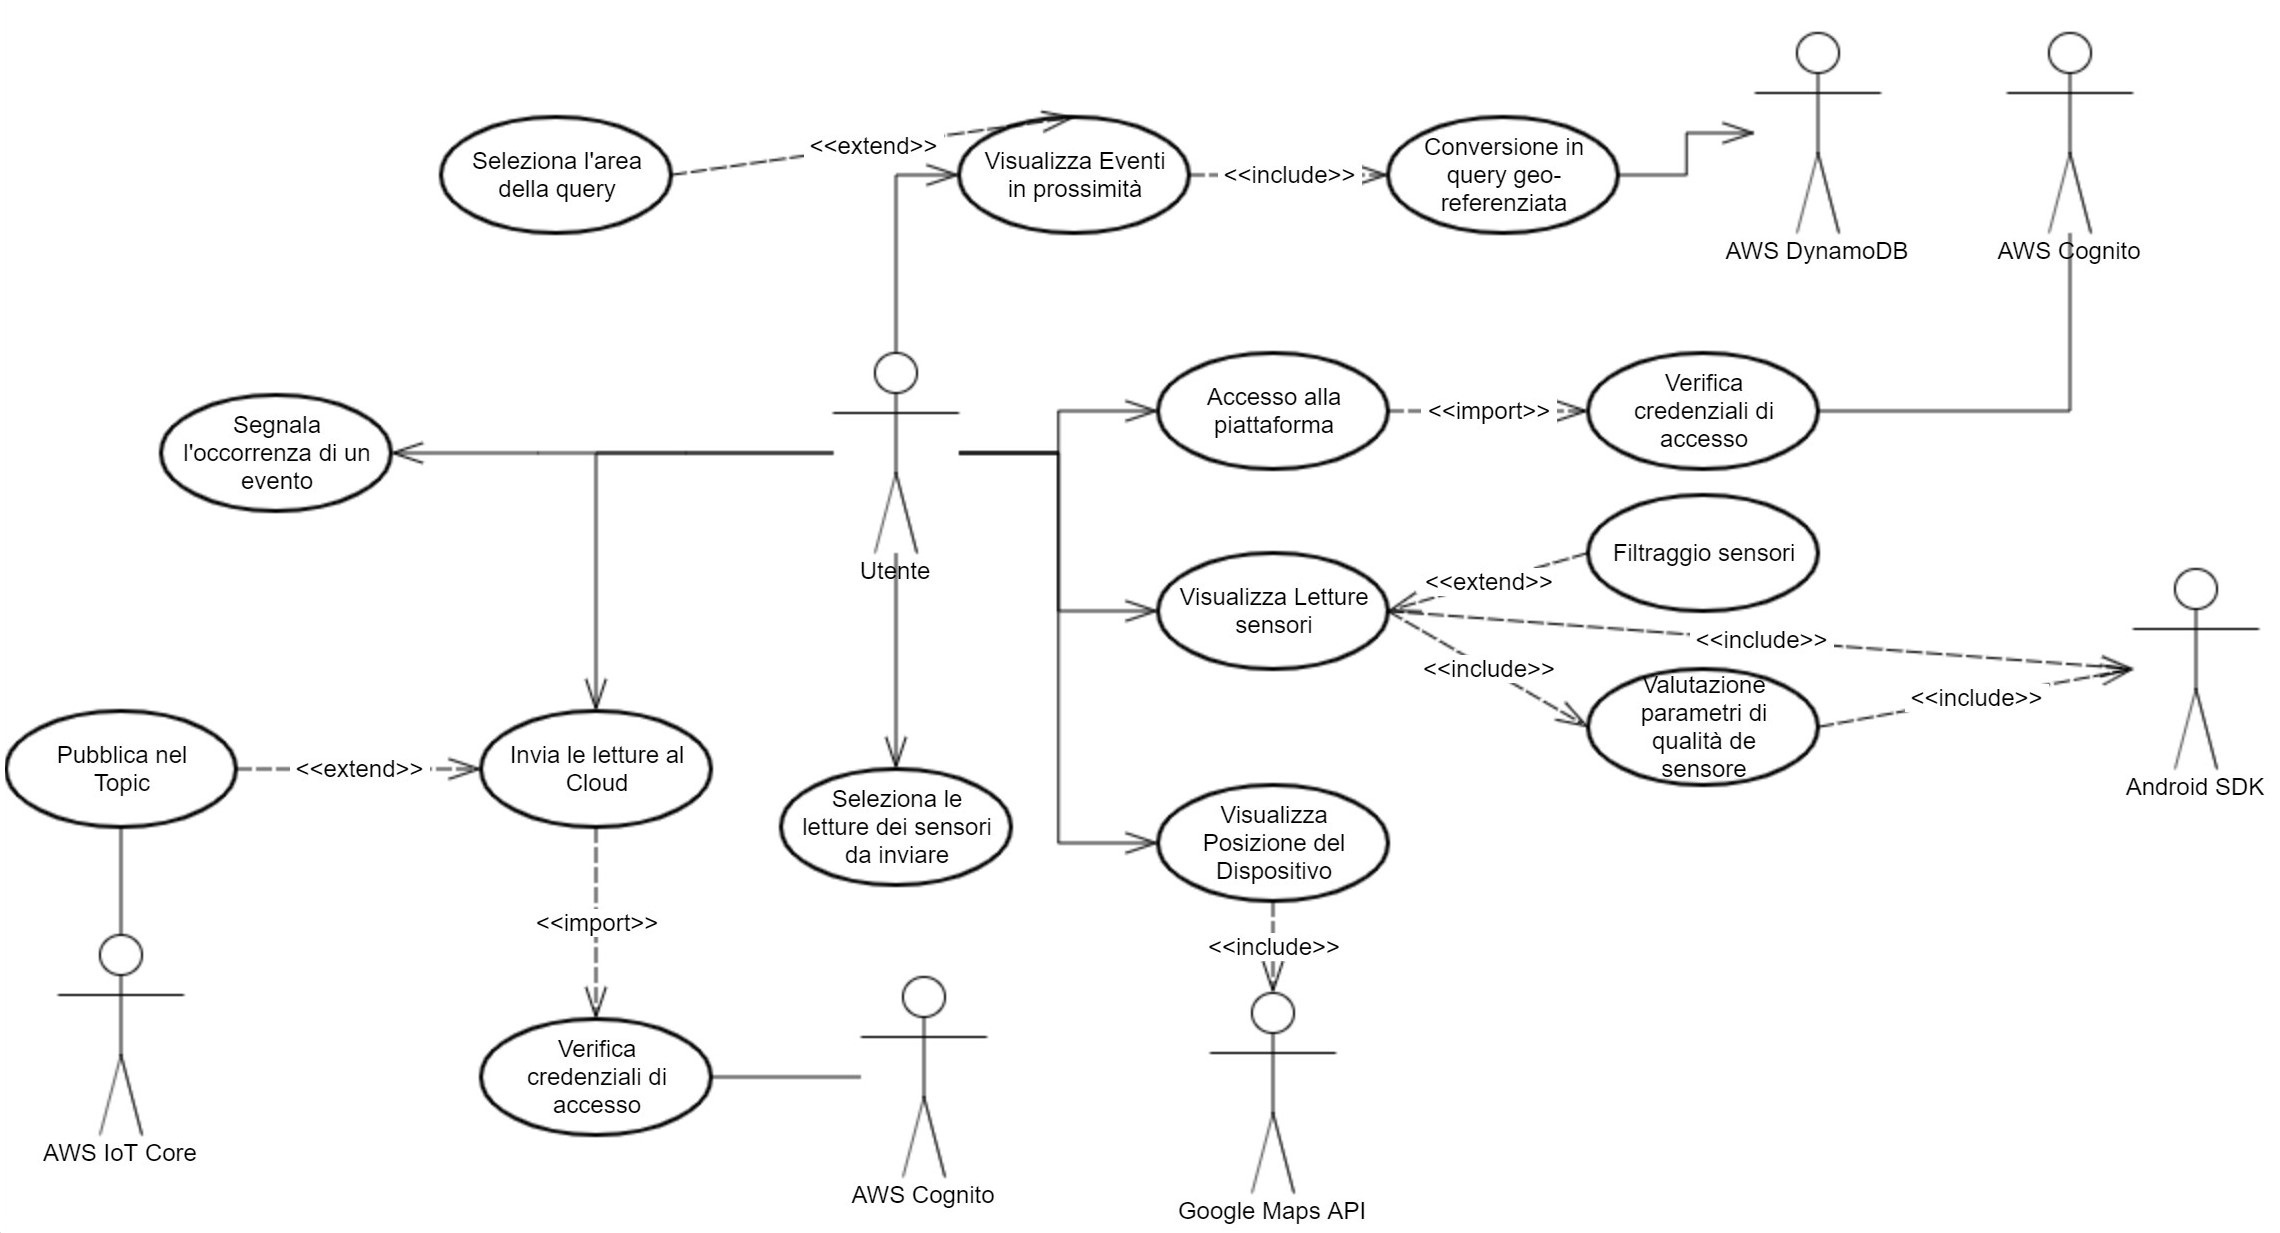
\includegraphics[width=1\columnwidth]{images/casiuso}
	\end{center}
	\caption{Diagramma dei casi d'uso elaborato sulla base dei requisiti funzionali del sistema \autoref{tabel:requisiti_software}}
	\label{fig:casiuso}
\end{figure}
Si procederà quindi per step all'implementazione delle singole componenti del sistema e nella fattispecie, l'ordine implementativo che sarà seguito è:
\begin{enumerate}
	\item Sviluppo della applicazione Android
	\item Sviluppo del Middleware IoT utilizzando la piattaforma AWS IoT Core
	\item Sviluppo delle tabelle nel Database AWS DynamoDB
\end{enumerate}

\section{Applicazione Android}
Per lo sviluppo della applicazione Android, si è scelto di utilizzare l'IDE Android Studio ed il linguaggio di programmazione JAVA. Di seguito, pertanto, utilizzando queste tecnologie saranno implementate le singole componenti della applicazione. Nella fattispecie, la struttura che si vuole dare alla Applicazione Andorid è mostrata in \autoref{fig:android_app_schema}.
In Android, ciascuna pagina di una applicazione Android contenente un riferimento al layout da mostrare all'utente ed un riferimento al codice JAVA associato alla pagina è chiamata Activity. Invece, un servizio utilizzato all'interno di una Activity viene chiamato Modulo. Ciascun modulo assolverà ad uno specifico compito. Pertanto, prima di passare alla implementazione di ogni Activity e Modulo della applicazione, si progetti lo schema generale che i vuole implementare.\\
\begin{figure}
	\begin{center}
		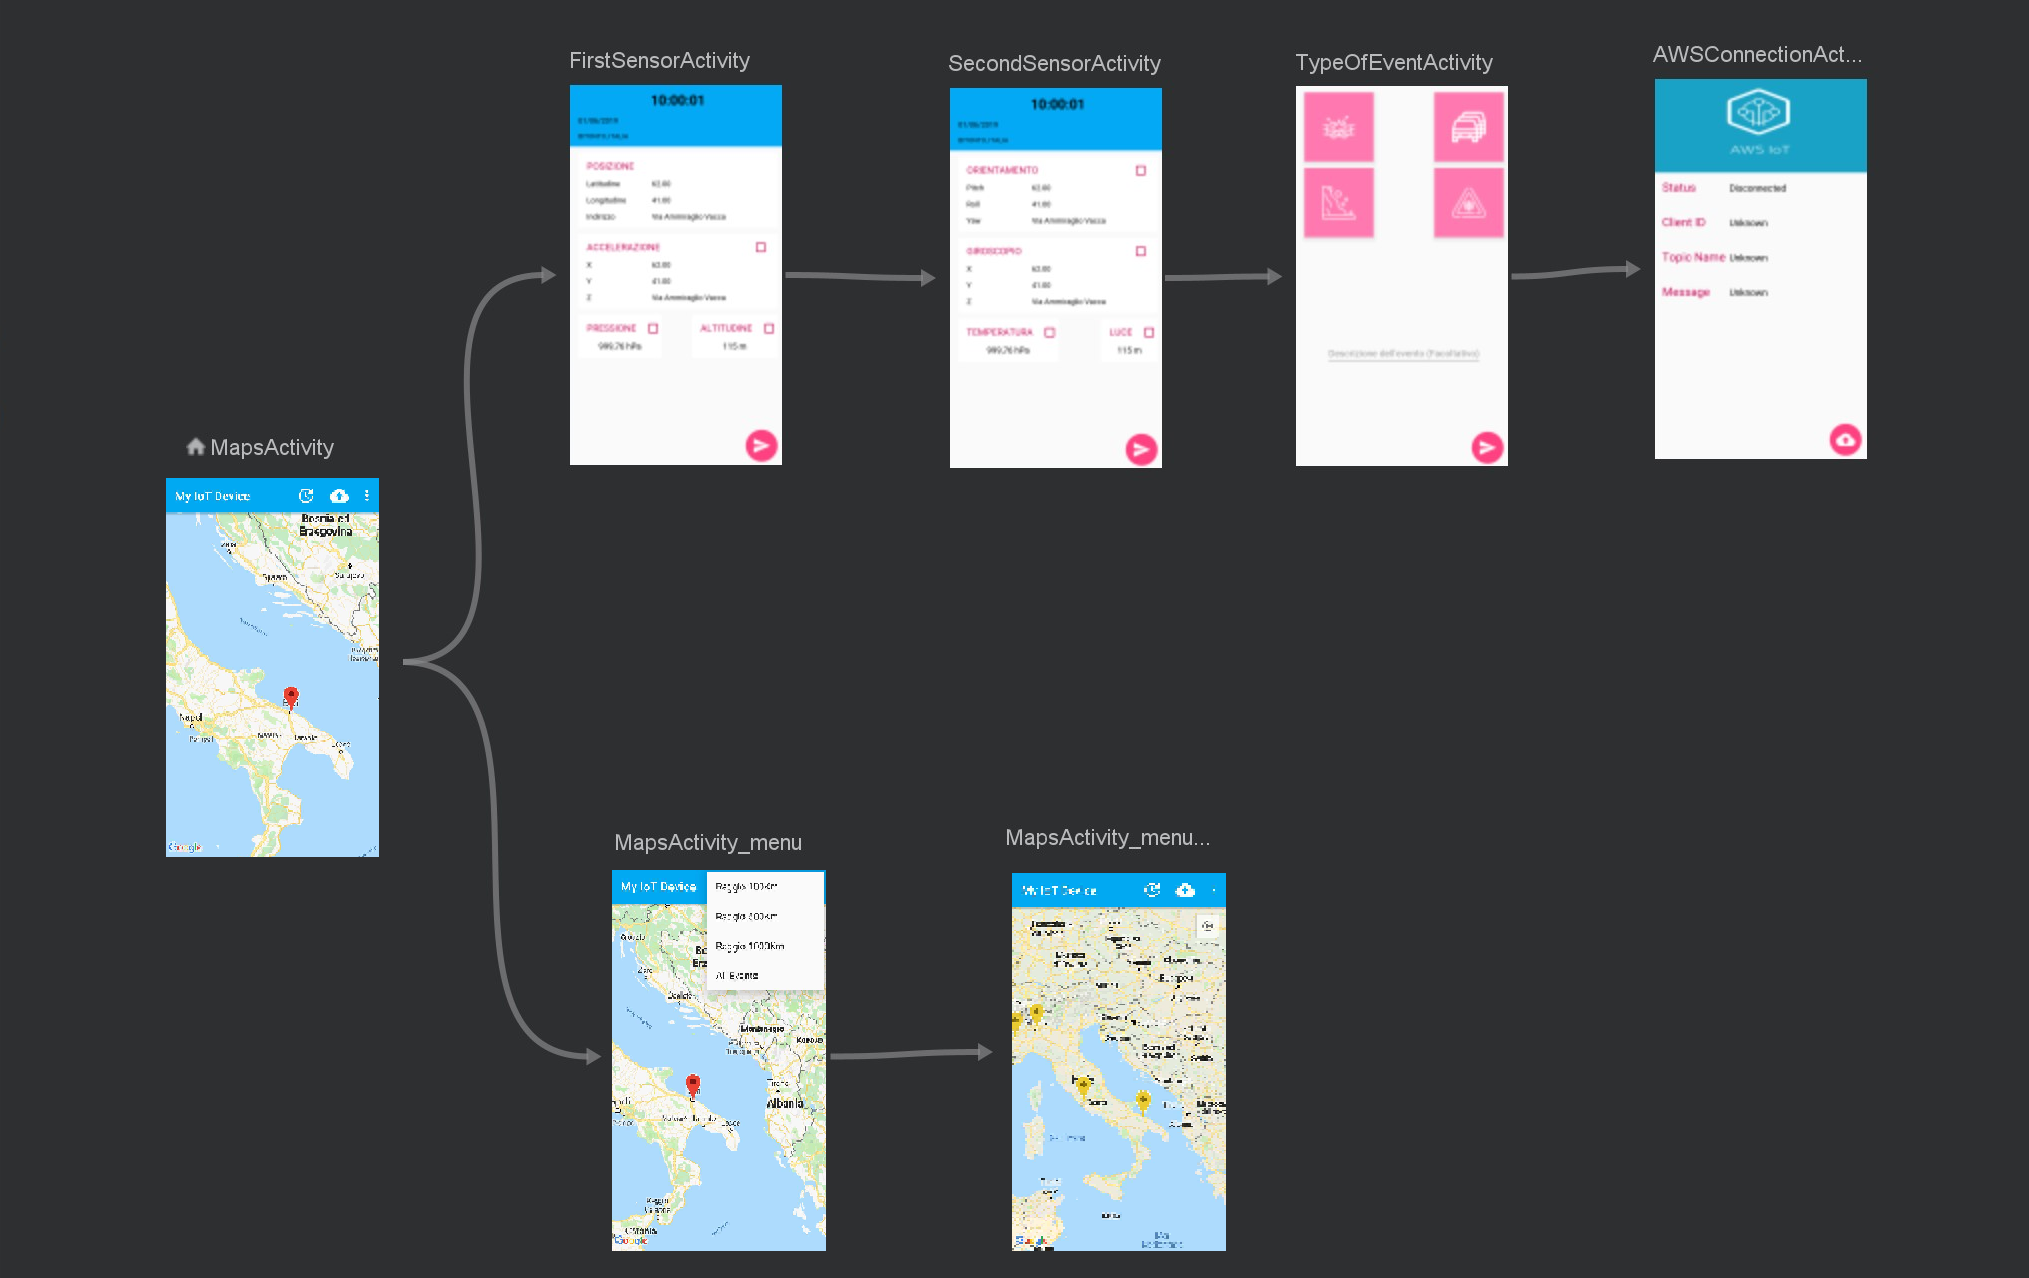
\includegraphics[width=1\columnwidth]{images/android_app_schema}
	\end{center}
	\caption{Schema delle Activity che compongono la applicazione Android}
	\label{fig:android_app_schema}
\end{figure}
\begin{figure}
	\begin{center}
		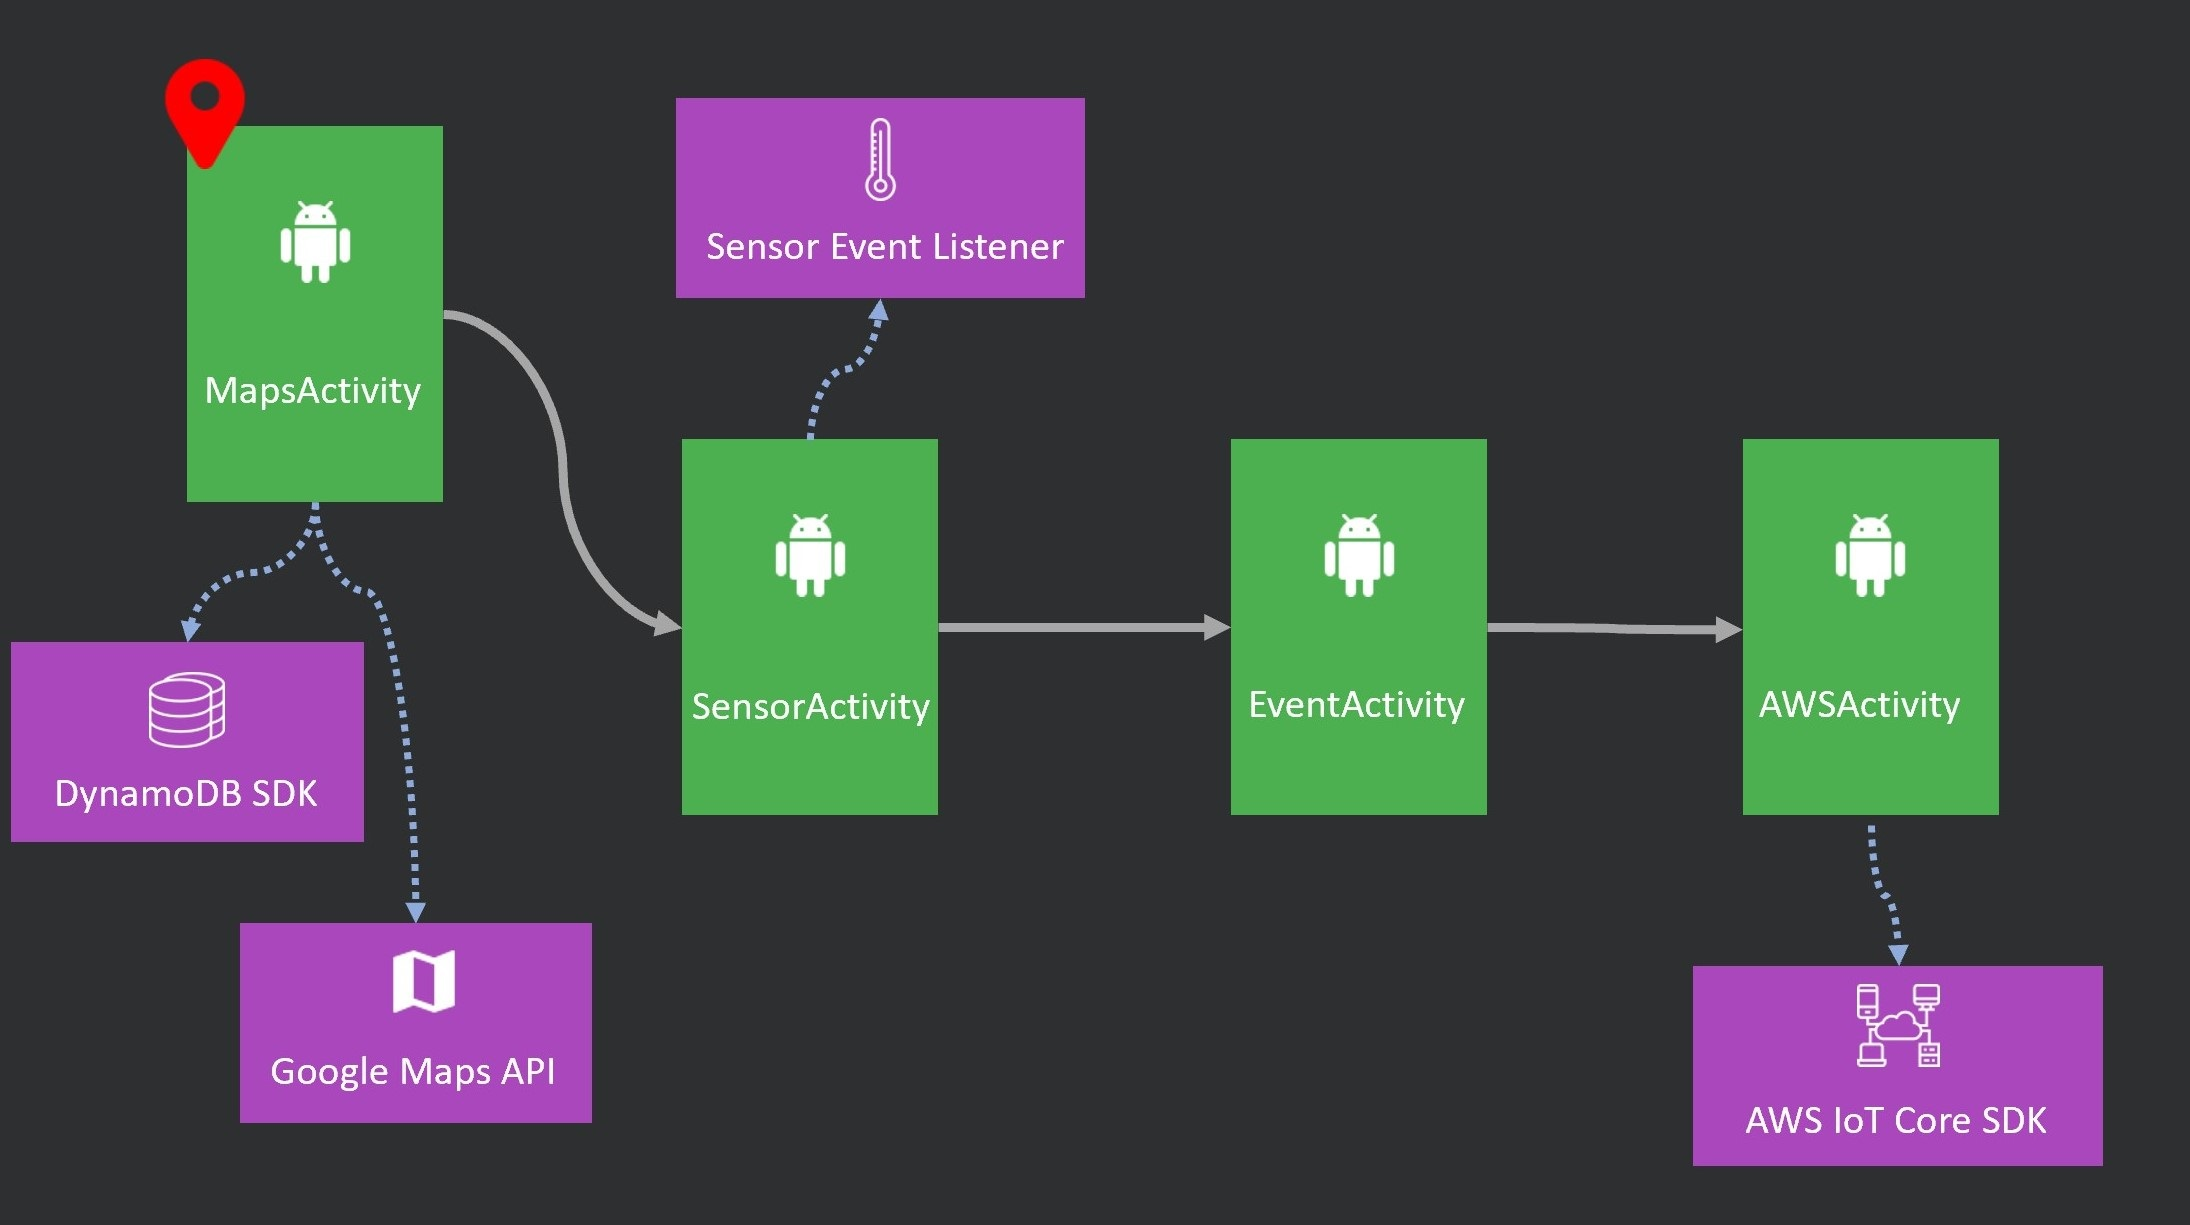
\includegraphics[width=0.9\columnwidth]{images/android_app_schema_1}
	\end{center}
	\caption{Moduli utilizzati da ciascuna Activity}
	\label{fig:android_app_schema_1}
\end{figure}
Dal momento che si è decsio di utilizzare l' IDE Android Studio, si proceda con la creazione di un nuovo progetto che quindi produrrà automaticamente lo schema della applicazione. Questo sarà lo scheletro della applicazione dal quale partire con l'implementazione di tutte le Activity ed i Moduli \autoref{fig:android_app}.
\begin{figure}
	\begin{center}
		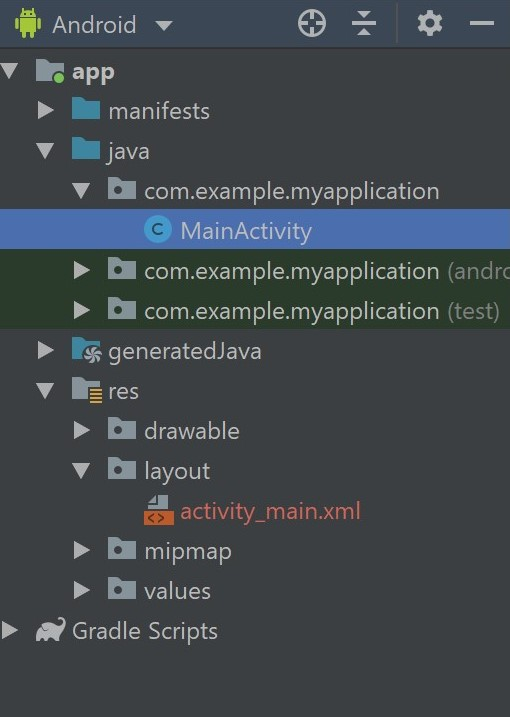
\includegraphics[width=0.3\columnwidth]{images/android_app}
	\end{center}
	\caption{Overview della nuova directory creata da Android Studio}
	\label{fig:android_app}
\end{figure}
Sono quindi mostrate nelle sezioni successive tutte le Activity che compongono la applicazione ed i rispettivi Moduli utilizzati.

\subsection{MapsActivity}
La MainActivity è quella che Android definisce come punto di partenza per il bootstrap o avvio di tutta la Applicazione. In questo caso, si vuole fare in modo che la prima Activity da mostrare all'utente sia la MapsActivity.\\
Lo scopo di questa Activity è quello di mostrare a schermo una mappa e, sfruttando la localizzazione GPS dello smartphone, di mostrare la posizione in tempo reale dell'utente sulla stessa mappa.\\
Ulteriormente, in questa Activity è necessario dare la possibilità all'utente di recuparare gli eventi conservati in una tabella di un Database DynamoDB (\autoref{fig:maps_activity}) attraverso una query geo-referenziata \textcolor{mypink}{1} e di mostrarli nella mappa attraverso dei marker \textcolor{mypink}{2}. Inoltre, accedendo al menù \textcolor{mypink}{3}, l'utente è in grado di modificare l'area degli eventi da recuperare dal Database.
\begin{figure}%
	\centering
	\subfloat[Componenti della MapsActivity]{{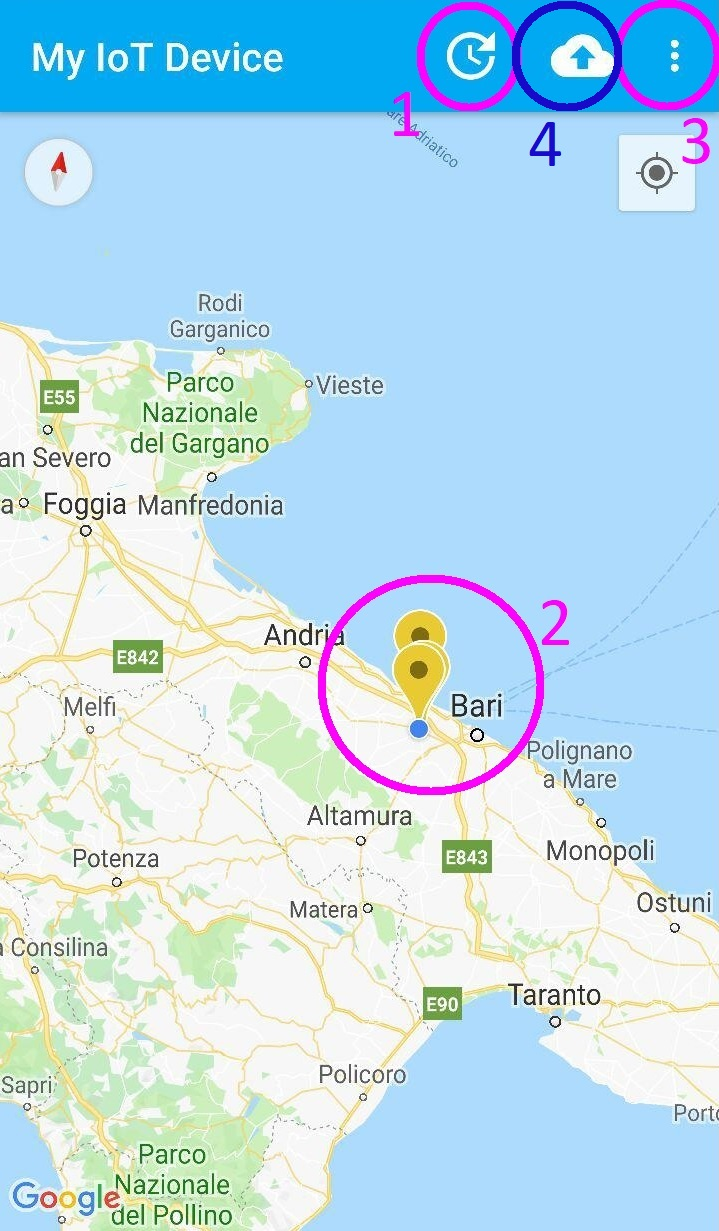
\includegraphics[width=5cm]{images/maps_activity_1} }}%
	\qquad
	\subfloat[Dettaglio del menù a tendina mostrato al click sul pulsante 3]{{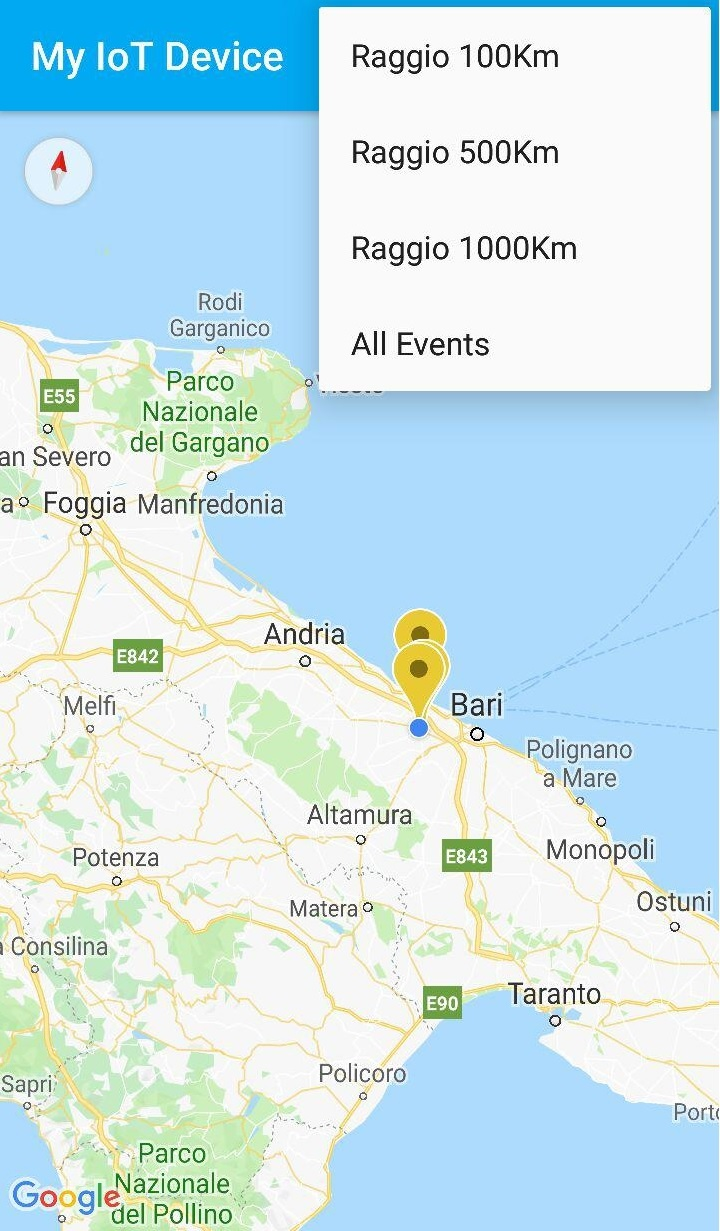
\includegraphics[width=5cm]{images/maps_activity_2} }}%
	\caption{Layout della Activity inziale nell'applicazione Android}%
	\label{fig:maps_activity}%
\end{figure}
In dettaglio, ad un click sul pulsante \textcolor{mypink}{3}, viene mostrato il menù a tendina che consente all'untente di selezionare la dimensione della query da inoltrare al Database.\\
Invece, un click sul pulsante \textcolor{blue}{4} consentirà all'utente di navigare verso le altre Activities che compongono la applicazione Android e nella fattispecie verso la SensorActivity che mostrerà a schermo le letture dei sensori dei quali lo smartphone è provvisto in real-time.\\
Di seguito, sono sposti gli step implementativi necessari alla realizzazione di questa Activity. Il codice relativo al layout di ciascuna applicazione è stato omesso in quanto non influisce direttamente sulle funzionalità implementate dalla applicazione stessa ed è ritenuto pertanto superfluo.

\subsubsection{Option Menu}
Per la creazione di un menù a tendina e per la conseguente gestione dei click sullo stesso è necessario:
\begin{itemize}
	\item \textit{Creare un nuovo layout del menu:} nella cartella \textbf{res} si crei una nuova cartella \textbf{menu} ed un nuovo file XML al suo interno. Questo file XML appena creato dovrà contenere il layout del menù a tendina da mostrare.
	
	\item \textit{Creare la MapsActivity.java ed associare i layout:} Nella cartella\\ \textbf{java/com.example.myapplication} si crei una nuova Activity che mostri a schermo il layout della mappa e quello del menu.
	\lstinputlisting[caption=Mostro a schermo il layout che ospiterà la mappa]{code/maps_activity_1.java}
	
	\item \textit{Gestire le interazioni dell'utente con il Menu:} Si rende necessario predisporre un listener in ascolto di eventuali iterazioni dell'utente con gli elementi del menù a tendina. In tal modo, al click su uno dei pulsanti del menù, si andrà ad aggiornare il valore dell'area della query e conseguentemente la query al database verrà reinviata per soddisfare le nuove richieste.
	\lstinputlisting[caption=Listener associato agli elementi del Menu]{code/maps_activity_2.java}
\end{itemize}

\subsubsection{GPS e Google Maps API}
Una volta creato il layout della applicazione, si implementi ora la componente che consente alla Activity di mostrare a schermo la posizione dell'utente nella mappa. Questa componente utilizzerà la posizione GPS dello smartphon per aggiornare in tempo reale una mappa. Inoltre, al fine di mostrare correttamente la mappa, è necessario sfruttare le API messe a disposizione da Google Maps.
\begin{itemize}
	\item \textit{Richiesta delle permission all'utente:} Si richiede all'utente il permesso di accedere alla posizione GPS ed alla connessione Internet del suo dispositivo. Il GPS sarà utilizzato per la posizione in real-time e la connessione ad internet sarà utilizzata per mostrare la Mappa.
	\lstinputlisting[caption=Accesso al GPS e connessione Internet]{code/permission.java}
	
	\item \textit{Utilizzo delle Google Maps API:} Al fine di mostrare a schermo una mappa è necessario ottenere una chiave API da Google Maps, previa registrazione al Web Service. Va pertanto creato un nuovo documento XML nella directory \textbf{res/google\_maps\_api.xml} e segire le istruzioni in \url{https://developers.google.com/maps/documentation/android/start#get-key} per ottenere una nuova chiave. Questa chiave andrà poi inserita all'interno del file XML appena creato.
	\lstinputlisting[caption=Utilizzo della chiave fornita da Google Maps per l'utilizzo delle Mappe]{code/google_map_api.xml}
		
	\item \textit{Aggiornamento in real time della view:} Sfruttando la posizione GPS e le Google Maps API, viene aggiornata in real-time la posizione dell'utente sulla mappa.
\end{itemize}

\subsubsection{Query del Database}
Infine, è necessario gestire le query da inviare al Database DynamoDB. Infatti, in funzione della scelta dell'utente sulla dimensione del raggio della query, verranno formulate delle query geo-referenziate al Database DynamoDB in modo da raccogliere i soli eventi segnalati nell'area prescelta.
\begin{itemize}
	\item \textit{Utilizzo l'SDK di DynamoDB:  }Viene sfruttato l'SDK messo a disposizione da AWS DynamoDB per mappare i dati contenuti nelle tabelle del database, sottoforma di classe all'interno dell'applicazione Android.
	\lstinputlisting[caption=Mapping delle tabelle ed attributi del Database DynamoDB che si vuole mappare]{code/dynamodb_3.java}
	
	\item \textit{Creazione di un task asincrono:} Viene utilizzato un task asincrono per l'interrogazione del database in modo da consentire all'utente di continuare ad usare l'interfaccia grafica anche durante le interrogazioni del Database.
	\lstinputlisting[caption=<struttura del Task Asincrono che dovrà interrogare il Database]{code/dynamodb_8.java}
	
	\item \textit{Composizione della Query:} Dovendo lanciare una query geo-referenziata e, dal momento che i dati nel database sono anch'essi geo-referenziati attraverso i campi latitudine e longitudine, è necessario ora unire le informazioni relative alla latitudie e longitudine corrente dell'utente con quelle relative al raggio della query. L'obiettivo di questo calcolo  quello di ottenere un intervallo di posizioni accettabili. Queste saranno caratterizzate dall'avere una latitudine e longitudine comprese all'interno di un certo intervallo.
	\lstinputlisting[caption=Calcolo dei parametri con i quali inviare una query geo-referenziata]{code/dynamodb_4.java}
	
	\item \textit{Invio della query geo-referenziata:} Sulla base del mapping effettuato tra gli attributi della tabella di DynamoDB e l'applicazione android, si può ora lanciare la query ed applicare il filtro sull'intervallo di posizioni che si vogliono raccogliere.
	\lstinputlisting[caption=Composizione ed invio della query]{code/dynamodb_5.java}
\end{itemize}

\subsubsection{Creazione di Marker sulla Mappa}
Una volta effettuata la query al Database DynamoDB, è necessario predisporre la ricezione della lista di tutti gli elementi che rispettano i parametri della query, decodificarli dal formato JSON nel quale sono trasmessi ad un formato più user-friendly e conseguentemente mostrarli a schermo sottoforma di marker nella mappa.
\begin{itemize}
	\item \textit{Ricevo la Lista di messaggi:} Inviata la query, mi aspetto di ricevere una lista di messaggi da parte del Database DynamoDB corrispondenti agli elementi all'interno del Database che soddisfano la query. 
	\lstinputlisting[caption=Ricezione degli item che soddisfano la query]{code/dynamodb_6.java}
	
	\item \textit{Creo un marker per ogni evento:} Ogni elemento ricevuto corrisponderà ad un evento geo-referenziato contenuto nel Database. Uso gli attributi latitudine e longitudine dell'evento per mostrarlo nella Mappa precedentemente creata.
	\lstinputlisting[caption=Visualizzazione di ciascun evento come marker sulla mappa]{code/dynamodb_7.java}
\end{itemize}

\subsection{SensorActivity}
La SensorActivity viene attivata ad un click dell'utente sul pulsante \textcolor{blue}{4} della \autoref{fig:maps_activity}. Lo scopo di questa Activity è quello di mostrare a schermo una panoramica delle letture restituite da tutti i sensori di cui è dotato lo smartphone per sottoporle ad una revisione dell'utente al fine di decidere quali di queste letture inviare al Server per le successive analisi. 
Dal momento che il panorama degli smartphone è notoriamente frammentato in termini di dotazione software ed hardware, si è deciso di predisporre una view per ogni sensore che potrebbe risultare utile alle successive analisi dei dati. Nella fattispecie, i sensori per cui sono stati predisposti i metodi necessari alla raccolta e visualizzazione dei dati sono:
\begin{itemize}
	\item Accelerazione
	\item Pressione Atmosferica
	\item Altimetro
	\item Orientamento
	\item Giroscopio
	\item Temperatura
	\item Intensità Luminosa
\end{itemize}
A prescindere dalla dotazione del dispositivo, si predisporranno i metodi utili ad ottenere le letture di questi sensori ove presenti. In caso uno dei sensori sopra citati dovesse non essere in dotazione dello smartphone, non ne sarà data alcuna lettura.
\begin{figure}%
	\centering
	\subfloat{{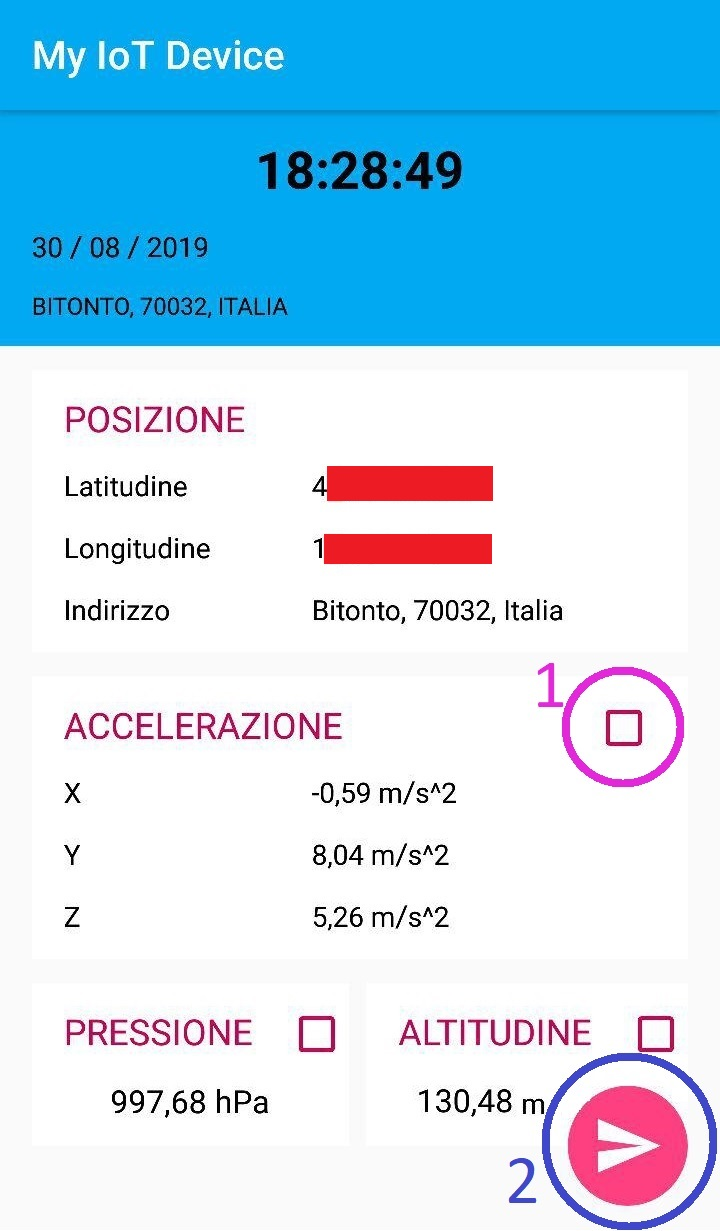
\includegraphics[width=5cm]{images/sensor_activity_1} }}%
	\qquad
	\subfloat{{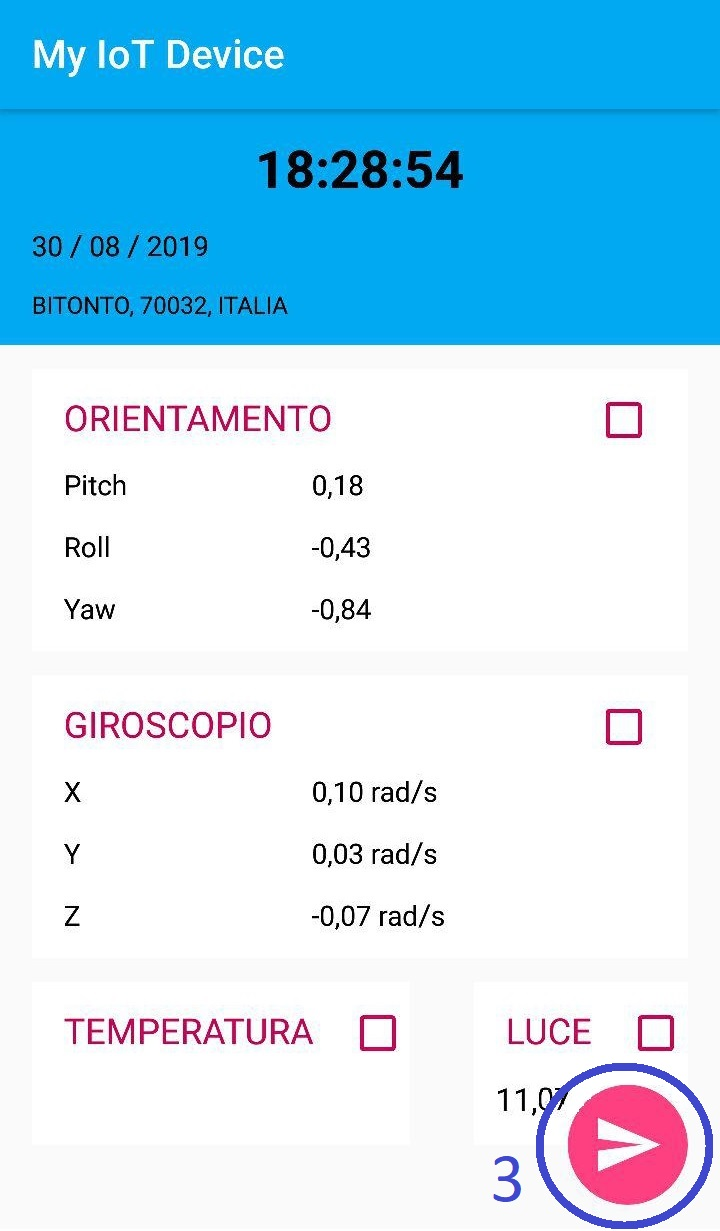
\includegraphics[width=5cm]{images/sensor_activity_2} }}%
	\caption{Lista Sensori con le relative misure}%
	\label{fig:sensor_activity}%
\end{figure}
Un click da parte dell'utente sulla CheckBox \textcolor{mypink}{1} consentrà di selezionare la lettura del relativo sensore da inviare al Middleware IoT. Cliccando invece sul FloatingButton \textcolor{blue}{2} si navigherà ad una SensorActivity gemella che mostrerà le letture di altri sensori. Infine, un click sul pulsante \textcolor{blue}{3}, farà navigare l'utente verso la Activity successiva (EventActivity).\\
Di seguito sono mostrati gli step per la visualizzazione dei dati di ciascun sensore. A titolo di esempio, questi step saranno mostrati per l'accelerometro ma potranno essere ripetuti per tutti gli altri sensori.
\begin{itemize}
	\item \textit{Creazione di un riferimento al SensorManager:} Al fine di ottenere l'accesso alle letture dei sensori, è necessario sfruttare un Modulo messo a disposizione dal framework Android chiamato SensorManager. Il SensorManager, si occuperà di disabilitare i sensori non necessari, specialmente quando la Activity è in pausa. Questo perchè il sistema non disattiva automaticamente i sensori quando lo schermo viene spento ne quando l'Activity viene messa in pausa e ciò si tradurrebbe in un eccessivo consumo della batteria.
	\lstinputlisting[caption=Creazione del riferimento al SensorManager che sarà condiviso tra tutti i sensori mostrati nella Activity]{code/sensor_1.java}
	
	\item \textit{Accesso alle risorse dello Smartphone:} Per ogni sensore che si intende utilizzare è necessario recuperare un riferimento al particolare sensore attraverso il SensorManager precedentemente istanzaiato. I diversi Sensori presenti all'interno di uno smartphone sono indivisuati dal SensorManager attraverso una lista di costanti accessibili da : \url{https://developer.android.com/guide/topics/sensors/sensors_overview}. In questo caso, si crei il riferimento all'accelerometro.
	\lstinputlisting{code/sensor_2.java}
	
	\item \textit{Creazione di un Thread separato:} Al fine di gestire le letture provenienti dal sensore e poterle inoltrare all'utente nella SensorActivity, è necessario creare un Thread separato rispetto a quello sul quale viene eseguita la SensorActivity. In questo modo, la SensorActivity sarà ancora disponibile all'utilizzo mentre un thread parallelo si starà procurando le letture dei sensori.
	\lstinputlisting[caption=Creazione e lancio del thread separato che leggerà i valori dall'accelerometro.]{code/sensor_3.java}
	
	\item \textit{Registrazione di un Listener sul Thread separato:} Al fine di recuperare e trattare i dati provenienti dal thread appena creato per l'accelerometro, è necessario creare e registrare un listener il cui compito è quello di eseguire delle operazioni sulle letture del sensore, nonappena sono ricevuti dei nuovi dati dal sensore stesso.
	\lstinputlisting[caption=Registrazione del Listener sull'accelerometro.]{code/sensor_4.java}
	\lstinputlisting[caption=Modulo Sensor Event Listener.]{code/sensor_5.java}
	
	\item \textit{Filtraggio dei dati in uscita dall'accelerometro:} Come evidenziato nella \autoref{subsec:filtering_sensor}, è necessario effettuare il filtraggio delle letture provenienti da alcuni sensori al fine i ottenere delle letture più accurate. L'accelerometro è tra quei sensori Hardware che richiedono un filtraggio dei dati.
	\lstinputlisting[caption=Funzione applicata all'output dell'accelerometro per il filtraggio dei dati con un filtro passa-basso.]{code/sensor_6.java}
	
	\item \textit{Stampa a schermo delle letture del sensore:} Una volta filtrati, i dati sono disponibili ad essere visualizzati nella SensorActivity.
	\lstinputlisting[caption=Accesso al contenuto degli elementi della view nella SensorActivity.]{code/sensor_7.java}
	
	\item \textit{Recupero dei parametri di qualità del sensore:} Per concludere con il processo di lettura dei dati di un sensore, è necessario corredare l'output del sensore con i parametri di qualità del sensore, la cui utilità è stata discussa nella \autoref{subsec:quality_param}.
	\lstinputlisting[caption=Lettura delle caratteristiche salienti del sensore.]{code/sensor_8.java}
\end{itemize}

\subsection{EventActivity}
\label{subsec:event_activity}
La EventActivity viene attivata ad un click dell'utente sul pulsante \textcolor{blue}{3} della \autoref{fig:sensor_activity}. Lo scopo di questa Activity è quello di mostrare a schermo una lista di possibili eventi stradali tra i quali l'utente può scegliere quelli eventualmente occorsi. Qualora infatti uno di questi eventi dovesse verificarsi lungo la rete stradale, l'utente può informare il sistema e di conseguenza tutti gli altri automobilisti dell'eventuale pericolo.
Infine si mette a disposizione anche una label per l'eventuale inserimento di una descrizione dell'evento \textcolor{mypink}{2}. Un click sul pulsante \textcolor{blue}{3} consentirà invece la navigazione verso la Activity successiva (AWSActivity).
\begin{figure}%
	\centering
	\subfloat[Componenti della EventActivity]{{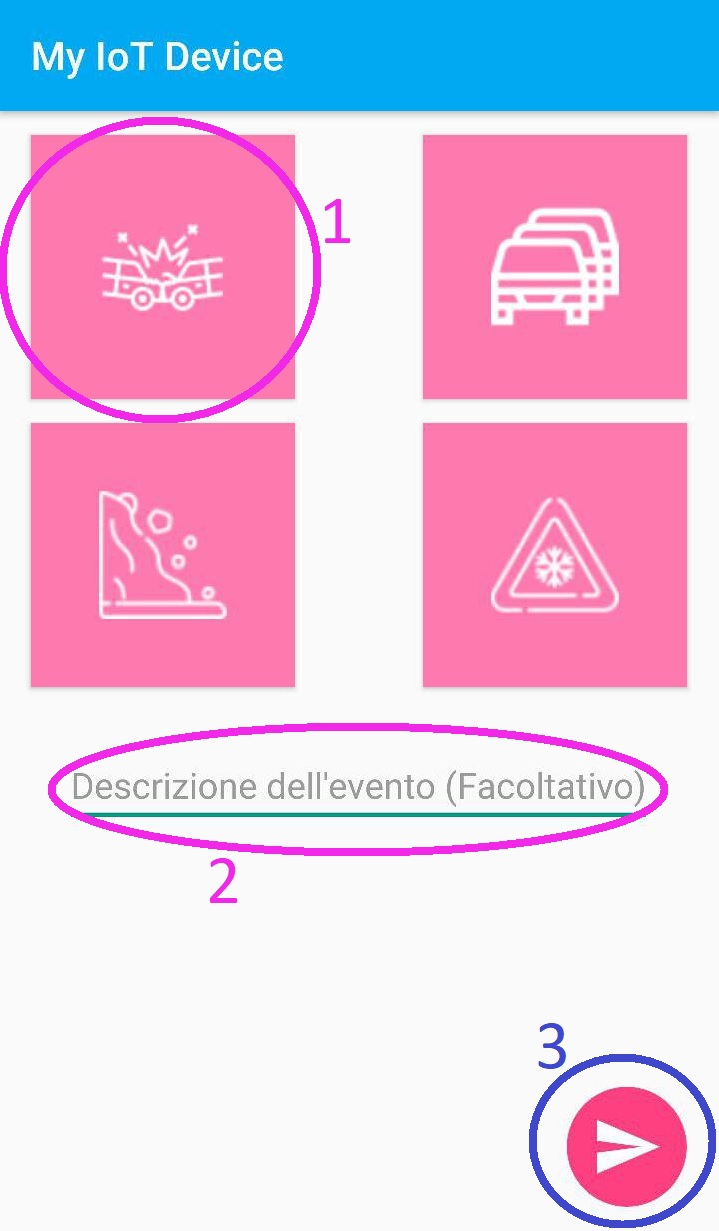
\includegraphics[width=5cm]{images/event_activity_1} }}%
	\qquad
	\subfloat[Dettaglio del click sul pulsante 1]{{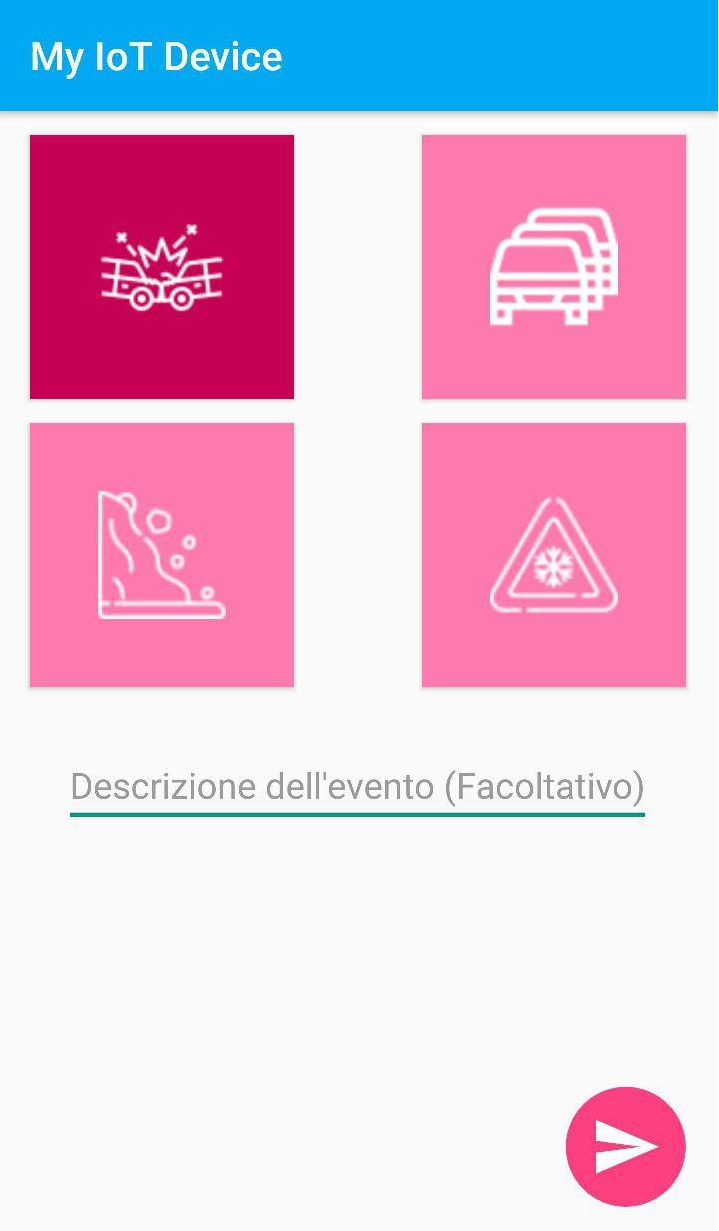
\includegraphics[width=5cm]{images/event_activity_2} }}%
	\caption{Layout della EventActivity}%
	\label{fig:event_activity}%
\end{figure}
Considerata la semplicità del contenuto da mostrare a schermo in questa Activity e considerato che questa sarà l'ultima Acivity a raccogliere i dati proposti dall'utente, conseguentemente al click dell'utente sul pulsante \textcolor{blue}{3} si creerà direttamente il payload del pacchetto da inviare nella Activity successiva (AWSActivity) in formato XML ed in formato JSON.\\
Per l'implementazione di queste componenti, sono stati seguiti gli step seguenti:
\begin{itemize}
	\item \textit{Gestire i click sui Pulsanti:} Per ciscun pulsante corrispondente ad un possibile evento stradale, viene predisposto un Listener che quindi resti in ascolto di interazioni con l'utente e si comporti di conseguenza.
	\lstinputlisting[caption=Gestione del click sul primo pulsante.]{code/event_1.java}
	
	\item \textit{Creazione della Publication in DATEX II:} In accordo con quanto definito dallo standard DATEX II che si è deciso di utilizzare come formato per lo scambio dati relativi al traffico, questi dati raccolti dall'utente saranno impacchettati in una Publication e conseguentemente convertiti in XML e JSON. Questa procedura è eseguita in questa Activity sulla base dello schema delle classi dell' \autoref{app:a} e sulla base dell'implementazione delle stesse evidenziata nell'\autoref{app:b}.
	
	\item \textit{Conversione della Publication in XML e JSON:} Android non prevede dei moduli integrati per la conversione di un oggetto in formato XML, ma solo in formato JSON. Pertanto, la conversione dell'oggetto Publication in formato XML sarà fatta utilizzando una libreria esterna. 
	\lstinputlisting[caption=Utilizzo della libreria XStream per la conversione della publication in formato XML.]{code/event_2.java}
	Per quanto riguarda invece la convesrione in formato JSON, sarà utilizzata la libreria Gson messa a disposizione da Android.
	\lstinputlisting[caption=Utilizzo della libreria Gson per la conversione della Publication in formato JSON.]{code/event_3.java}
\end{itemize}

\subsection{AWSActivity}
\label{subsec:aws_activity}
La AWS Activity viene attivata ad un click dell'utente sul pulsante \textcolor{blue}{3} della \autoref{fig:event_activity}.
\begin{figure}%
	\centering
	\subfloat[Componenti della AWSActivity]{{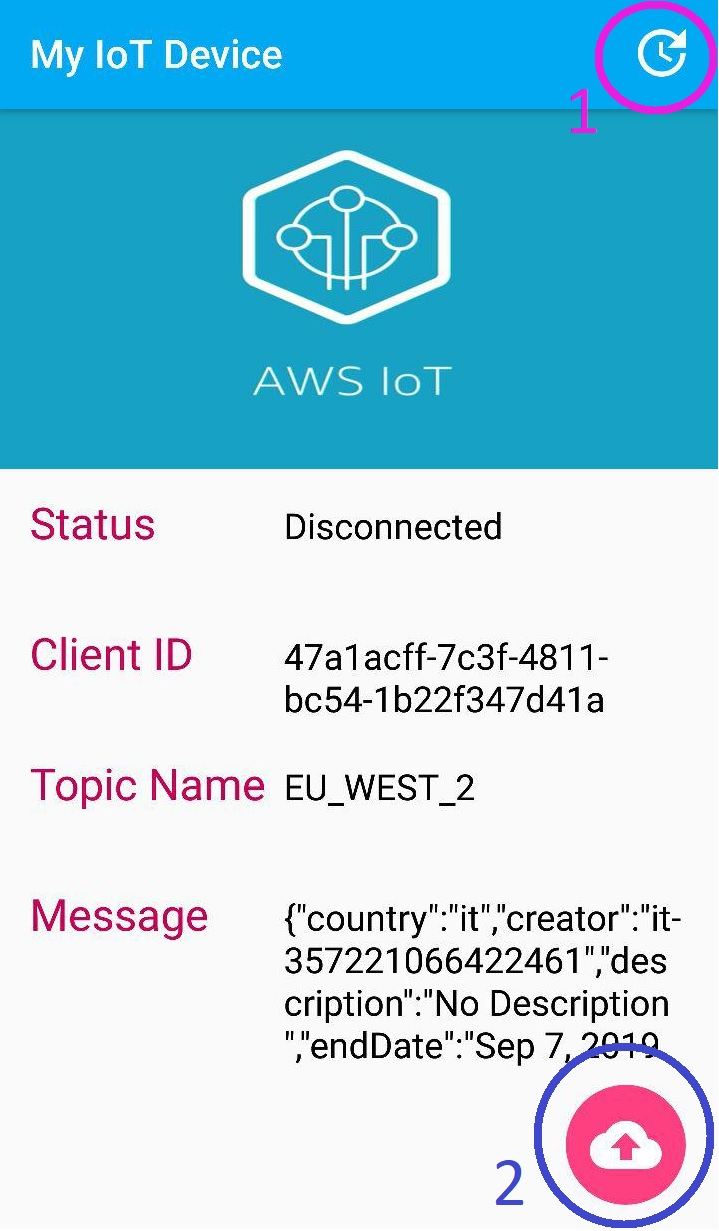
\includegraphics[width=5cm]{images/aws_activity_1} }}%
	\qquad
	\subfloat[Dettaglio del click sul pulsante 1]{{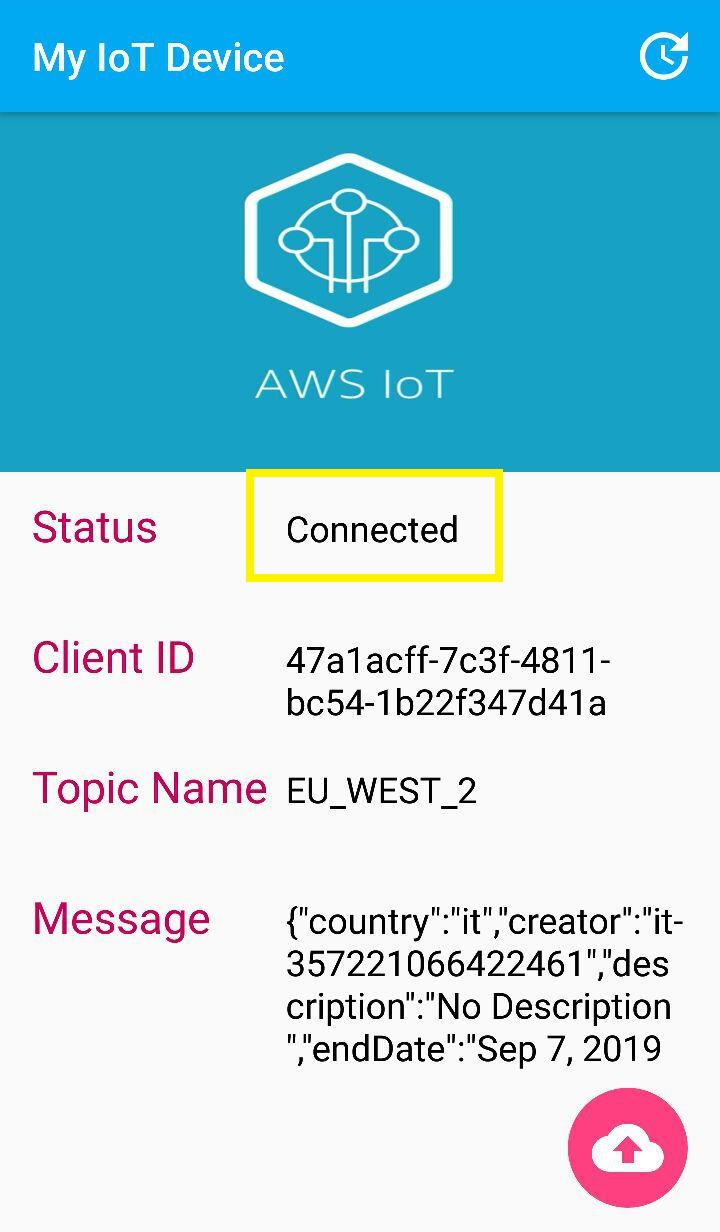
\includegraphics[width=5cm]{images/aws_activity_2} }}%
	\caption{Layout della AWSActivity}%
	\label{fig:aws_activity}%
\end{figure}
Lo scopo di questa Activity è quello di stabilire una connessione con la piattaforma Cloud AWS IoT Core attraverso un click sul pulsante \textcolor{mypink}{1} e, una volta stabilita la connessione, procedere all'invio del messaggio al Middleware IoT con un click sul pulsante \textcolor{blue}{2}. \\
Le funzionalità associate a questa Activity potrebbero essere tranquillamente incorporate in un click sul pulsante \textcolor{blue}{3} della \autoref{fig:event_activity}. Tuttavia, ai fini della prototipazione, si è scelto di tenere queste funzionalità in una Activity separata in modo da mostrarne in dettaglio le singole operazioni.
La sequenza di operazioni eseguite in questa Activity saranno quindi:
\begin{itemize}
	\item \textit{Set-Up dei parametri necessari alla Connessione:} Al fine di stabilire la connessione con il Server AWS IoT Core, è necessario che ciascun Client sia registrato al servizio Amazon Web Services e che quindi abbia un ID ed una Password per il proprio accesso. In questa fase prototipale, il processo di registrazione è stato fatto manualmente seguendo la procedura esposta nella \autoref{sec:iot_core}. Le credenziali di accesso ottenute in questo processo di registrazione saranno utilizzate per l'autorizzazione della applicazione in fase di sviluppo alla comunicazione con il server.
	\lstinputlisting[caption=Variabili necessarie alla autenticazione del Client.]{code/aws_1.java}
	
	\item \textit{Creazione del ClientID:} La trasmissione dei dati tra la applicazione android Client ed il Server AWS IoT Core avverrà utilizzando il protocollo MQTT il quale richiede un Client ID univoco. Tale Client ID viene generato automaticamente da una funzione randomica.
	\lstinputlisting[caption=Generazione di un Client ID.]{code/aws_2.java}
	
	\item \textit{Autenticazione attraverso AWS Cognito:} AWS Cognito è lo strumento che consente di aggiungere strumenti di registrazione, accesso e controllo sugli accessoi in applicazioni Web e dispositivi mobili. In automatico quindi, si andrà a registrare il dispositivo ad AWS Cognito per l'accesso ad AWS IoT Core tramite le credenziali di accesso precedentemente registrate nella AWSActivity.
	\lstinputlisting[caption=Utilizzo di AWS Cognito per l'accesso ad AWS IoT Core.]{code/aws_3.java}
	
	\item \textit{Stabilire la Connessione con il Server:} Una volta implementati i metodi messi a disposizione dall'AWS SDK per garantire l'accesso alla applicazione android, si gestisce ora il click sul pulsante \textcolor{mypink}{1} per la creazione di una connessione con il server.
	\lstinputlisting[caption=Connsessione con l'AWS IoT Core.]{code/aws_4.java}
	
	\item \textit{Invio del messaggio:} In conclusione, una volta stabilita la connessione, l'utente può cliccare sul pulsante \textcolor{blue}{2} per l'invio del pacchetto al Server.
	\lstinputlisting[caption=Invio della Publication al Server.]{code/aws_5.java}	
\end{itemize}

\section{AWS IoT Core}
\label{sec:aws_core}
Nella \autoref{subsec:aws_dev} si è mostrato come procedere alla registrazione ed utilizzo della piattaforma AWS IoT Core, tuttavia se ne sono volutamente omessi alcuni dettagli implementativi per essere trattati in questa sezione, in modo da avere una migliore panoramica sulla struttura della Applicazione e sulla tipologia dei messaggi inviati.
Si è visto quindi come registrarsi al servizio e come fare in modo che IoT Core sia in ascolto su un predefinito topic e che tutti i client che vogliano comunicare con il server, debbano pubblicare messaggi sullo stesso topic nel quale il server è in ascolto.\\
Nella \autoref{subsec:aws_dev} e nella \autoref{subsec:aws_activity} si è fatto sempre riferimento a pubblicazioni sul topic denominato \textbf{EU\_WEST\_2} senza tuttavia spiegarne il motivo. \\
Si rende necessario introdurre una feature di AWS IoT Core per la quale viene creata una console indipendente (o Server) per ogni area geografica. Questo significa che, un dispositivo in una data area geografica, avrà un topic ad esso corrispondente (che in questo caso è appunto \textbf{EU\_WEST\_2}) e quindi potrà inviare i dati solo al topic corrispondente. In questo modo IoT Core riesce a garantire una buona scalabilità e delle ottime prestazioni anche in corrispondenza di un numero molto elevato di dispositivi. \\
Questa suddivisione granulare dei topic e dei server in ascolto sui diversi topic facilita anche l'interfacciamento con il Database e facilita analogamente l'invio di query geo-referenziate al Database.
Infatti, attraverso questa granularità sarà possibile implementare un diverso Database DynamoDB associato a ciascun server in ascolto su ciascun topic in modo da estendere la scalabilità di cui gode AWS IoT Core anche al database DynamoDB.
In questo modo, infatti, una query da parte di un utente appartenente ad una data area geografica (e quindi con uno specifico Topic) sarà riferita ad un singolo e specifico Database DynamoDB che conterrà i dati relativi a quella sola area geografica. \\
Tuttavia, qualora necessario, nulla vieta ad un utente di interrogare tutti gli altri Database DynamoDB relativi ad altre aree geografiche. Eventualmente, queste interrogazioni su diversa scala, possono anche essere regolamentate da diversi processi di autenticazione e che quindi solo alcuni utenti possano interrogare Database diversi rispetto a quello relativo alla propria area geografica.
\begin{figure}
	\begin{center}
		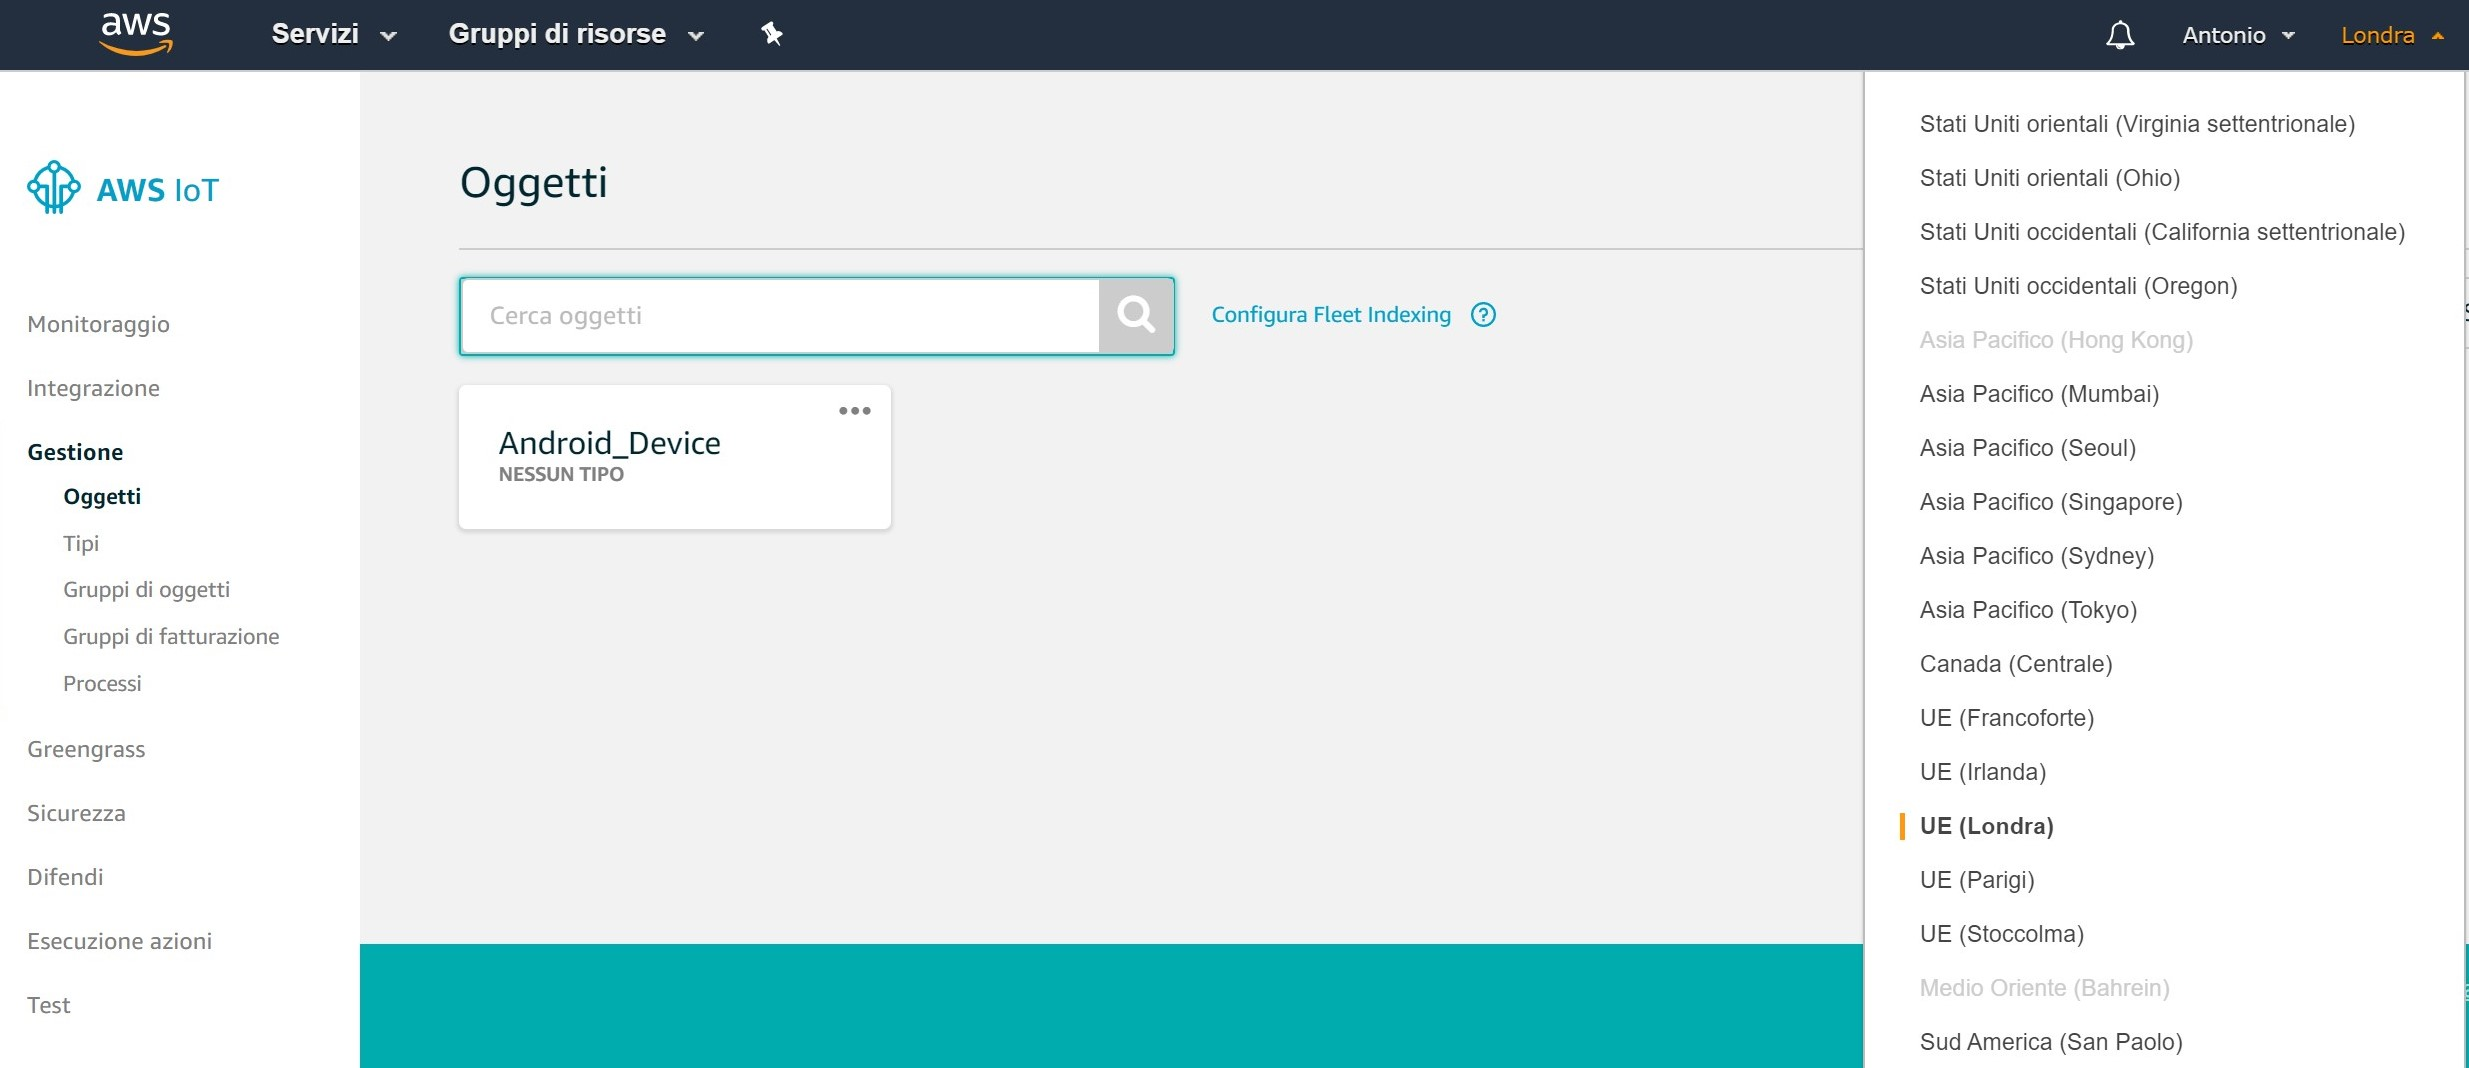
\includegraphics[width=0.9\columnwidth]{images/aws_1}
	\end{center}
	\caption{Lista di tutti i topic supportati da AWS IoT Core suddivisi per area geografica.}
	\label{fig:aws_1}
\end{figure}
Un'altro vantaggio di questa separazione tra i server che sono in ascolto sui diversi topic e quindi sulle diverse aree geografiche, consiste nel fatto che gli oggetti 'shadow' creati su un server (come spiegato nella \autoref{subsec:aws_dev}), sono relativi solo a quel server in ascolto su quel topic in quell'area geografica. In questo modo, è possibile creare oggetti diversi in aree geografiche diverse in funzione eventualmente delle diverse disponibilità, necessità e standard utilizzati in ciascuna area geografica.\\
Ulteriormente, così come gli oggetti sono relativi ad una singola area geografica o topic, anche le regole di AWS IoT Core lo saranno. Nella \autoref{subsec:dynamodb} si era infatti implementata una regola che consentisse al Middleware IoT Core di inviare ogni nuovo dato ricevuto avente come topic \textbf{EU\_WEST\_2} ad una tabella del database di DynamoDB.
\begin{figure}
	\begin{center}
		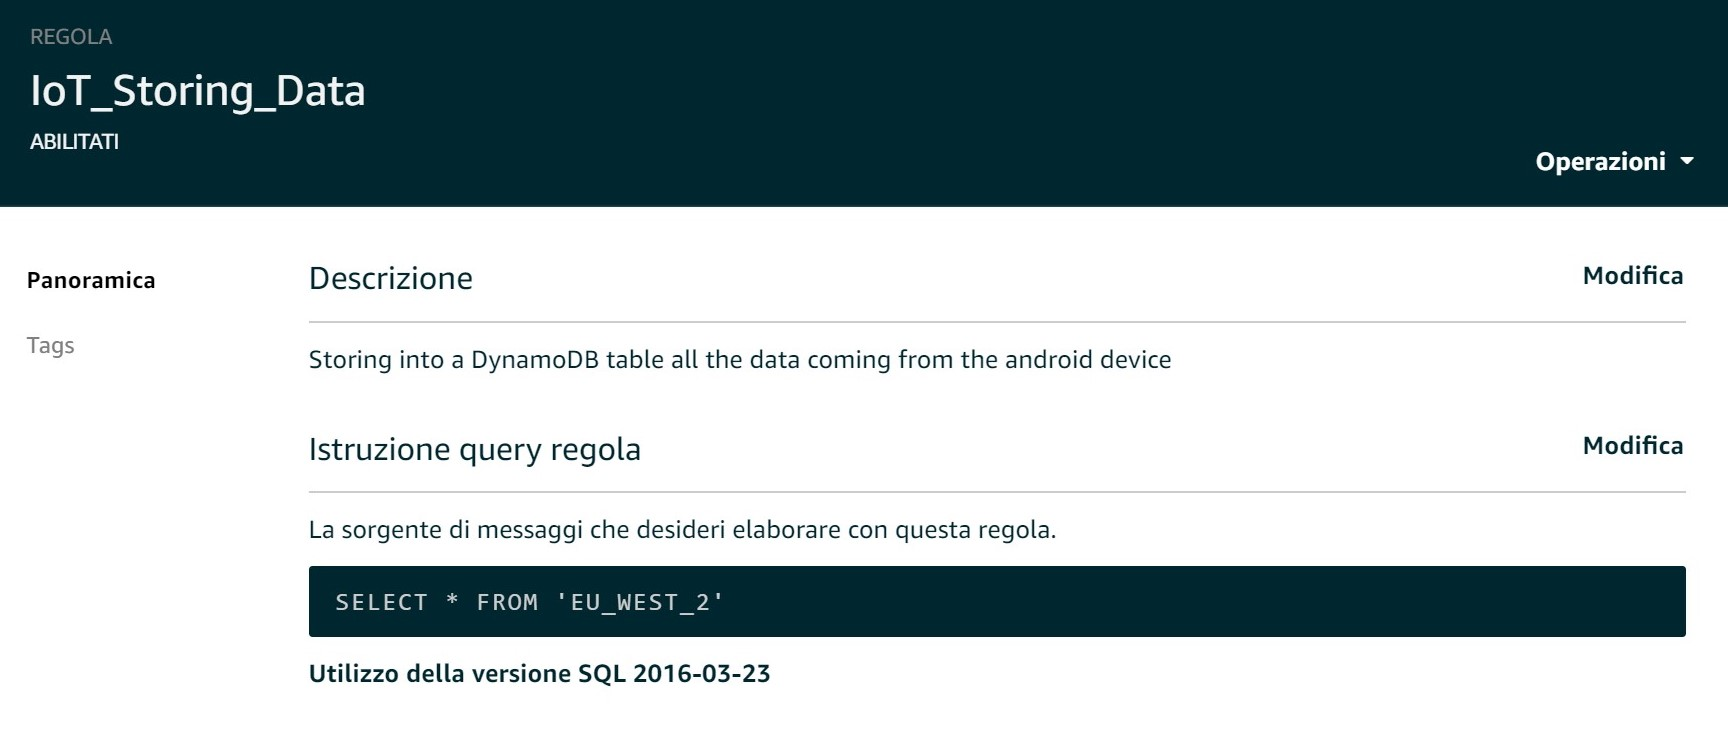
\includegraphics[width=0.7\columnwidth]{images/dynamodb_3}
	\end{center}
	\caption{Regola per la scrittura sul Database DynamoDB}
	\label{fig:dynamodb_31}
\end{figure}
Questa regola sarà ovviamente valida per il solo server IoT Core in ascolto sul topic \textbf{EU\_WEST\_2} mentre, per gli altri server in ascolto su altri topic potrà essere seguita la stessa procedura mostrata nella \autoref{subsec:dynamodb} con il riferimento ad un diverso topic.
Le nuove regole svilupate potranno, ove ritenuto opportuno, inserire i loro dati all'interno della stessa tabella di DynamoDB, ovvero all'interno della stessa tabella nella quale inserisce i dati anche la regola mostrata in \autoref{fig:dynamodb_31}. Alternativamente, i dati potranno essere inseriti all'interno di diverse tabelle nello stesso database o ancora potranno essere inseriti in una diversa tabella di un diverso database. Certamente questo ultimo caso si rende ideale per garantire delle performance migliori e si rende adatto a realizzare l'architettura descritta in \cite{famous:paper_detti_1}.
Tuttavia, nel prototipo realizzato in questo lavoro di tesi si è scelto per semplicità di implementare la prima soluzione. In questo modo, una singola tabella di un singolo databse in DynamoDB conterrà tutti i dati relativi a tutti i topic.


\section{DynamoDB}
Come ultima componente, resta da implementare la struttura del database in DynamoDB. La procedura che è stata seguita è quella descritta nella \autoref{subsec:dynamodb}. Questa stessa procedura può essere seguita per la creazione di diverse tabelle in diversi Database relativi a diversi topic. \\
L'ultima considerazione da effettuare riguarda il formato nel quale i dati sono memorizzati all'interno del Database ed inviati allo stesso.
Nella \autoref{subsec:event_activity} si è ritenuto opportuno convertire (o serializzare) il payload del messaggio (o publication) da inviare al middleware IoT Core in formato XML ed in formato JSON. Questa dopiia serializzazione dello stesso payload è effettuata in modo da poter mostrare in output, sottoforma di file di testo, il payload del messaggio in formato XML, come da Standard DATEX II. Un esempio di output è mostrato nell' \autoref{app:b} per evidenziare la corrispondenza tra il payload generato dalla applicazione ed il payload richiesto dallo Standard DATEX II.\\
Tuttavia, sebbene il middleware IoT AWS Core supporti messaggi in formato XML, il database DynamoDB, essendo un database NoSQL memorizza i dati sottoforma di coppie chiave-valore e quindi in formato JSON. 
Questo problema potrebbe essere risolto inviando il payload in formato XML fino al middleware IoT Core, effettuare la conversione dall'XML al JSON ed infine memorizzare il payload in formato JSON all'interno del Database. Tuttavia, questo procedimento di riconversione risulterebbe più lento e dispendioso rispetto alla genereazione e trasmissione dei dati direttamente in formato JSON. Per questo motivo, già all'interno della applicazione android viene generato il payload in fromato JSON.
\lstinputlisting[caption=Payload del messaggio in fromato JSON.]{code/payload.json}
